% -------------------------------------------------------------------------- %
% Style is derived from the tufte-handout style available on GitHub at
% https://github.com/Tufte-LaTeX/tufte-latex
% License: Apache 2.0
\documentclass[nohyper, % Turn off defaults, customize hyperref locally
               ]{tufte-handout}

% -------------------------------------------------------------------------- %
% Define document-specific macros here
\newcommand{\release}{0.14\xspace} % Update with new version
\DeclareRobustCommand{\ski}{\texttt{scikit-image}\xspace}
\DeclareRobustCommand{\spy}{SciPy\xspace} % Sadly, \sp is reserved (superscript)
\DeclareRobustCommand{\np}{NumPy\xspace}
\newcommand{\eg}{e.g.\xspace}
\newcommand{\rgb}{\textcolor{DarkRed}{R}\textcolor{DarkGreen}{G}\textcolor{DarkBlue}{B}}
\newcommand*{\vcenteredhbox}[1]{\begingroup
\setbox0=\hbox{#1}\parbox{\wd0}{\box0}\endgroup}
\newcommand{\pyblue}[1]{\textcolor{DarkBlue}{\pyv{#1}}}


% -------------------------------------------------------------------------- %
% Definitions used throughout the package
\title{\ski: the image processing toolkit for \spy}
\author[the \ski contributors]{the \ski contributors}
\date{9 July 2018} % Specify date, or comment out to use current date


% -------------------------------------------------------------------------- %
% Slightly tweak page layout so title fits on one line
\newgeometry{textwidth=27pc,      % 1pc wider than default
             marginparwidth=11pc, % 1pc narrower than default
             left=1in,
             top=1in,
             headsep=2\baselineskip,
             marginparsep=2pc,
             textheight=45\baselineskip,
             headheight=\baselineskip}


% Layout debugging
% \usepackage{showframe} % uncomment to debug page layout


% -------------------------------------------------------------------------- %
% Begin!
\begin{document}

\maketitle% tufte-handout command: prints title, author, and date

% Stay on brand
\begin{marginfigure}[-0.1cm]%
  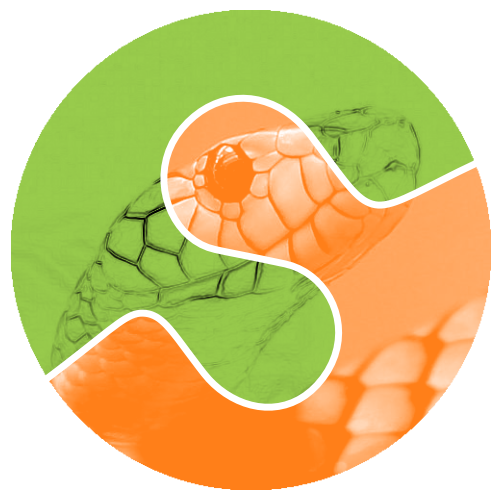
\includegraphics[width=\linewidth]{green_orange_snake.png}
  \label{fig:skimage_logo}
\end{marginfigure}

% Explain purpose
Welcome to \ski! This handout is designed to supplement and enhance the \ski tutorial materials, hosted on GitHub at \url{http://github.com/scikit-image/skimage-tutorials}. Our goal is to orient you to the package and provide you with a quick reference to common functions, so you can be as productive as possible!

\subsection{Where are my functions?} % (fold)
  \label{sec:Where_are_my_functions}
  Most of the functionality in \ski\marginnote[-0.1cm]{Unlike \textsc{matlab}, functions are grouped into \textit{subpackages} in \ski.} is located in \textit{subpackages}. This is similar to how \spy works. The reverse side of this handout has details about \ski subpackages available in version \release.
  % section Where_are_my_functions (end)

\subsection{Images are arrays} % (fold)
  \label{sub:images_are_arrays}

  \begin{marginfigure}[0.4cm]%
    \includegraphics[width=\linewidth]{tux_inset.png}
    \label{fig:tux_inset}
  \end{marginfigure}

  An image is simply a collection of data on a regular, often two-dimensional grid. In \ski, we use \np arrays to represent images. Color images have more than one channel, \eg, red, green, and blue (\rgb). Thus, the \np array for a color image is \textit{three}-dimensional, with channel information in the final dimension.
  % subsection images_are_arrays (end)

\subsection{Speak our language} % (fold)
  \label{sub:talking_our_language}
  To avoid confusion, we refrain from using the terms \textit{x} or \textit{y}. Throughout the package, \ski refers to \textit{rows} (r) and \textit{columns} (c). When color data is present, \textit{channel} (ch) denotes the third dimension. \np arrays representing 2D images are indexed via \pyv{arr[rows, columns]}.
  %
  \begin{marginfigure}[-1.1cm]%
    \includegraphics[width=\linewidth]{row-col.png}
    \label{fig:row-col}
  \end{marginfigure}
  % subsection talking_our_language (end)

\subsection{Additional resources} % (fold)
  \label{sub:additional_resources}
  The \ski website is located at \url{skimage.org/docs/stable}, including an API reference, user guide, and a gallery of examples. Development and issue tracking occur on the GitHub project page \url{github.com/scikit-image/scikit-image}. Pull requests are welcome!\\\medskip
  %
  \begin{marginfigure}[-1.7cm]%
    \centering%
    \begingroup
      \vcenteredhbox{
\includegraphics[height=0.59cm]{GitHub-Mark-Large.png}}%
      \vcenteredhbox{
\includegraphics[height=1cm]{GitHub-Logo.png}}%
    \endgroup
    \label{fig:GitHub}%
  \end{marginfigure}%
  %
  \noindent
  Interact with the community in the \ski Gitter chat room at \url{gitter.im/scikit-image/scikit-image} or post to the Google Group at \url{groups.google.com/forum/#!forum/scikit-image}.
  % subsection additional_resources (end)

\subsection{A humble request} % (fold)
  \label{sub:a_humble_request}
  Please cite the \ski paper\cite{van2014scikit} if you find this package useful! Citations allow developers to justify continued work on \ski.
  % subsection a_humble_request (end)

% -------------------------------------------------------------------------- %
% Reverse side: Road map to the package
\newpage%
\section{Road map to \ski} % (fold)
  \label{sec:road_map}
  Brief descriptions of every subpackage in \ski \release follow. Each subpackage contains algorithms used for similar purposes.\\

  % Horizontal line
  \noindent%
  \begingroup%
    \begin{center}%
      \textcolor{DarkGray}{\rule{0.7\textwidth}{.4pt}}\\%
    \end{center}%
  \endgroup%

  % Astronaut test image example
  \begin{marginfigure}[0cm]%
    \includegraphics[width=\linewidth]{astronaut.png}%
    \label{fig:astronaut}%
  \end{marginfigure}%
  %
  \begin{description}%
    \item[skimage.color] Color conversions.
    \begin{description}
      \item[rgb2gray] Convert a red-green-blue (\rgb) color image to grayscale.
    \end{description}
    \item[skimage.data] Test images.
    \begin{description}
      \item[astronaut] Image of the astronaut Eileen Collins\footnote[2][-0.2cm]{The \textcolor{DarkBlue}{\texttt{astronaut}} test image, an excellent public domain test image.}.
    \end{description}
    \item[skimage.draw] Drawing primitives such as lines or text.
    \item[skimage.exposure] Intensity and contrast adjustments.
    \item[skimage.feature] Feature detection and extraction.
    \begin{description}
      % Blob finding example
      \begin{marginfigure}[-0.3cm]%
        \includegraphics[width=\linewidth]{doh_galaxies.png}%
        \label{fig:doh_galaxies}%
      \end{marginfigure}%
      %
      \item[ORB] Used in the panorama tutorial along with \pyblue{match_descriptors}.
      \item[blob_*] Tunable blob detectors\footnote[3][0.1cm]{Blob detection in the Hubble Deep Field with \textcolor{DarkBlue}{\texttt{blob\_doh}}.}.
    \end{description}
    \item[skimage.filters] Whole-image changes like sharpening. \hfill \\See also the rank filters in \pyblue{skimage.filters.rank}.
    \item[skimage.future] The bleeding edge, with potentially unstable API.
    \item[skimage.graph] Graph theory, shortest paths.
    \item[skimage.io] Read (\pyblue{imread}), save (\pyblue{imsave}), and display images.
    \item[skimage.measure] Quantify image properties (length, shape).
    \begin{description}
      % Hough transform example
      \begin{marginfigure}[-3.3cm]%
        \includegraphics[width=\linewidth]{hough_lines.png}%
        \label{fig:hough_lines}%
      \end{marginfigure}%
      %
      \item[hough_line] Find lines in an image\footnote[4][-0.7cm]{Hough transforms can detect lines (above), circles, or ellipses.}. Circle, ellipse also available.
    \end{description}
    \item[skimage.morphology] Morphological operations, \eg, dilation and erosion. Binary and grayscale morphology supported.
    \item[skimage.novice] Simplified teaching interface.
    \item[skimage.restoration] Remove noise or deconvolve images.
    \item[skimage.segmentation] Partition an image into multiple regions.
    \begin{description}
      % Felzenszwalb segmentation example
      \begin{marginfigure}[-1.5cm]%
        \includegraphics[width=\linewidth]{felzenszwalb.png}%
        \label{fig:felzenszwalb}%
      \end{marginfigure}%
      %
      \item[felzenszwalb] Segment based on local contrast\footnote[5][0.05cm]{Automated segmentation using \textcolor{DarkBlue}{\texttt{felzenszwalb}}'s method.}. \hfill \\See also: \pyblue{slic}, \pyblue{quickshift}, and \pyblue{random_walker}.
    \end{description}
    \item[skimage.transform] Warp or rotate images.
    \begin{description}
      % Affine transformation example
      \begin{marginfigure}[0.1cm]%
        \includegraphics[width=\linewidth]{warp_affine.png}%
        \label{fig:affine}%
      \end{marginfigure}%
      %
      \item[warp] Geometric and affine\footnote[6][0.05cm]{\textcolor{DarkBlue}{\texttt{PiecewiseAffineTransform}} applied to the \textcolor{DarkBlue}{\texttt{astronaut}} with \textcolor{DarkBlue}{\texttt{warp}}.} transformations, a variety of which are exposed in this subpackage.
    \end{description}
    \item[skimage.util] Common public utility functions.
    \begin{description}
      \item[pad/crop] Image padding/cropping.
    \end{description}
    \item[skimage.viewer] QT-based interactive GUI.
  \end{description}
  % section road_map (end)

% -------------------------------------------------------------------------- %
% Dummy page, exists only so BibTeX can run (and gets trimmed)
\newpage
% Bibliography
\bibliography{bibliography}
\bibliographystyle{plainnat}

\end{document}
